\chapter{Dataset}
In questo capitolo si presentano le simulazioni ottenute da due taskset con una complessità maggiore rispetto a quelli del Capitolo~\ref{cap:implementazione}.

%%%%%%%%%%%%%%%%%%%%%%%%%%%%%%%%%%%%%%%%%%%%%%%%%%%%%%%%%%%%
\section{Taskset 1}
Il primo taskset complesso, mostrato in Figura~\ref{fig:dataset1} è composto da 5 task senza risorse condivise ed è quindi schedulato da Earliest Deadline First (EDF). Il taskset in questione ha un fattore di utilizzo della CPU di 0,95 e solo due task sono puramente periodici. Per introdurre la stocasticità ed aumentare la complessità della simulazione si campiona l'execution time dei chunk.

\begin{figure}[htbp]
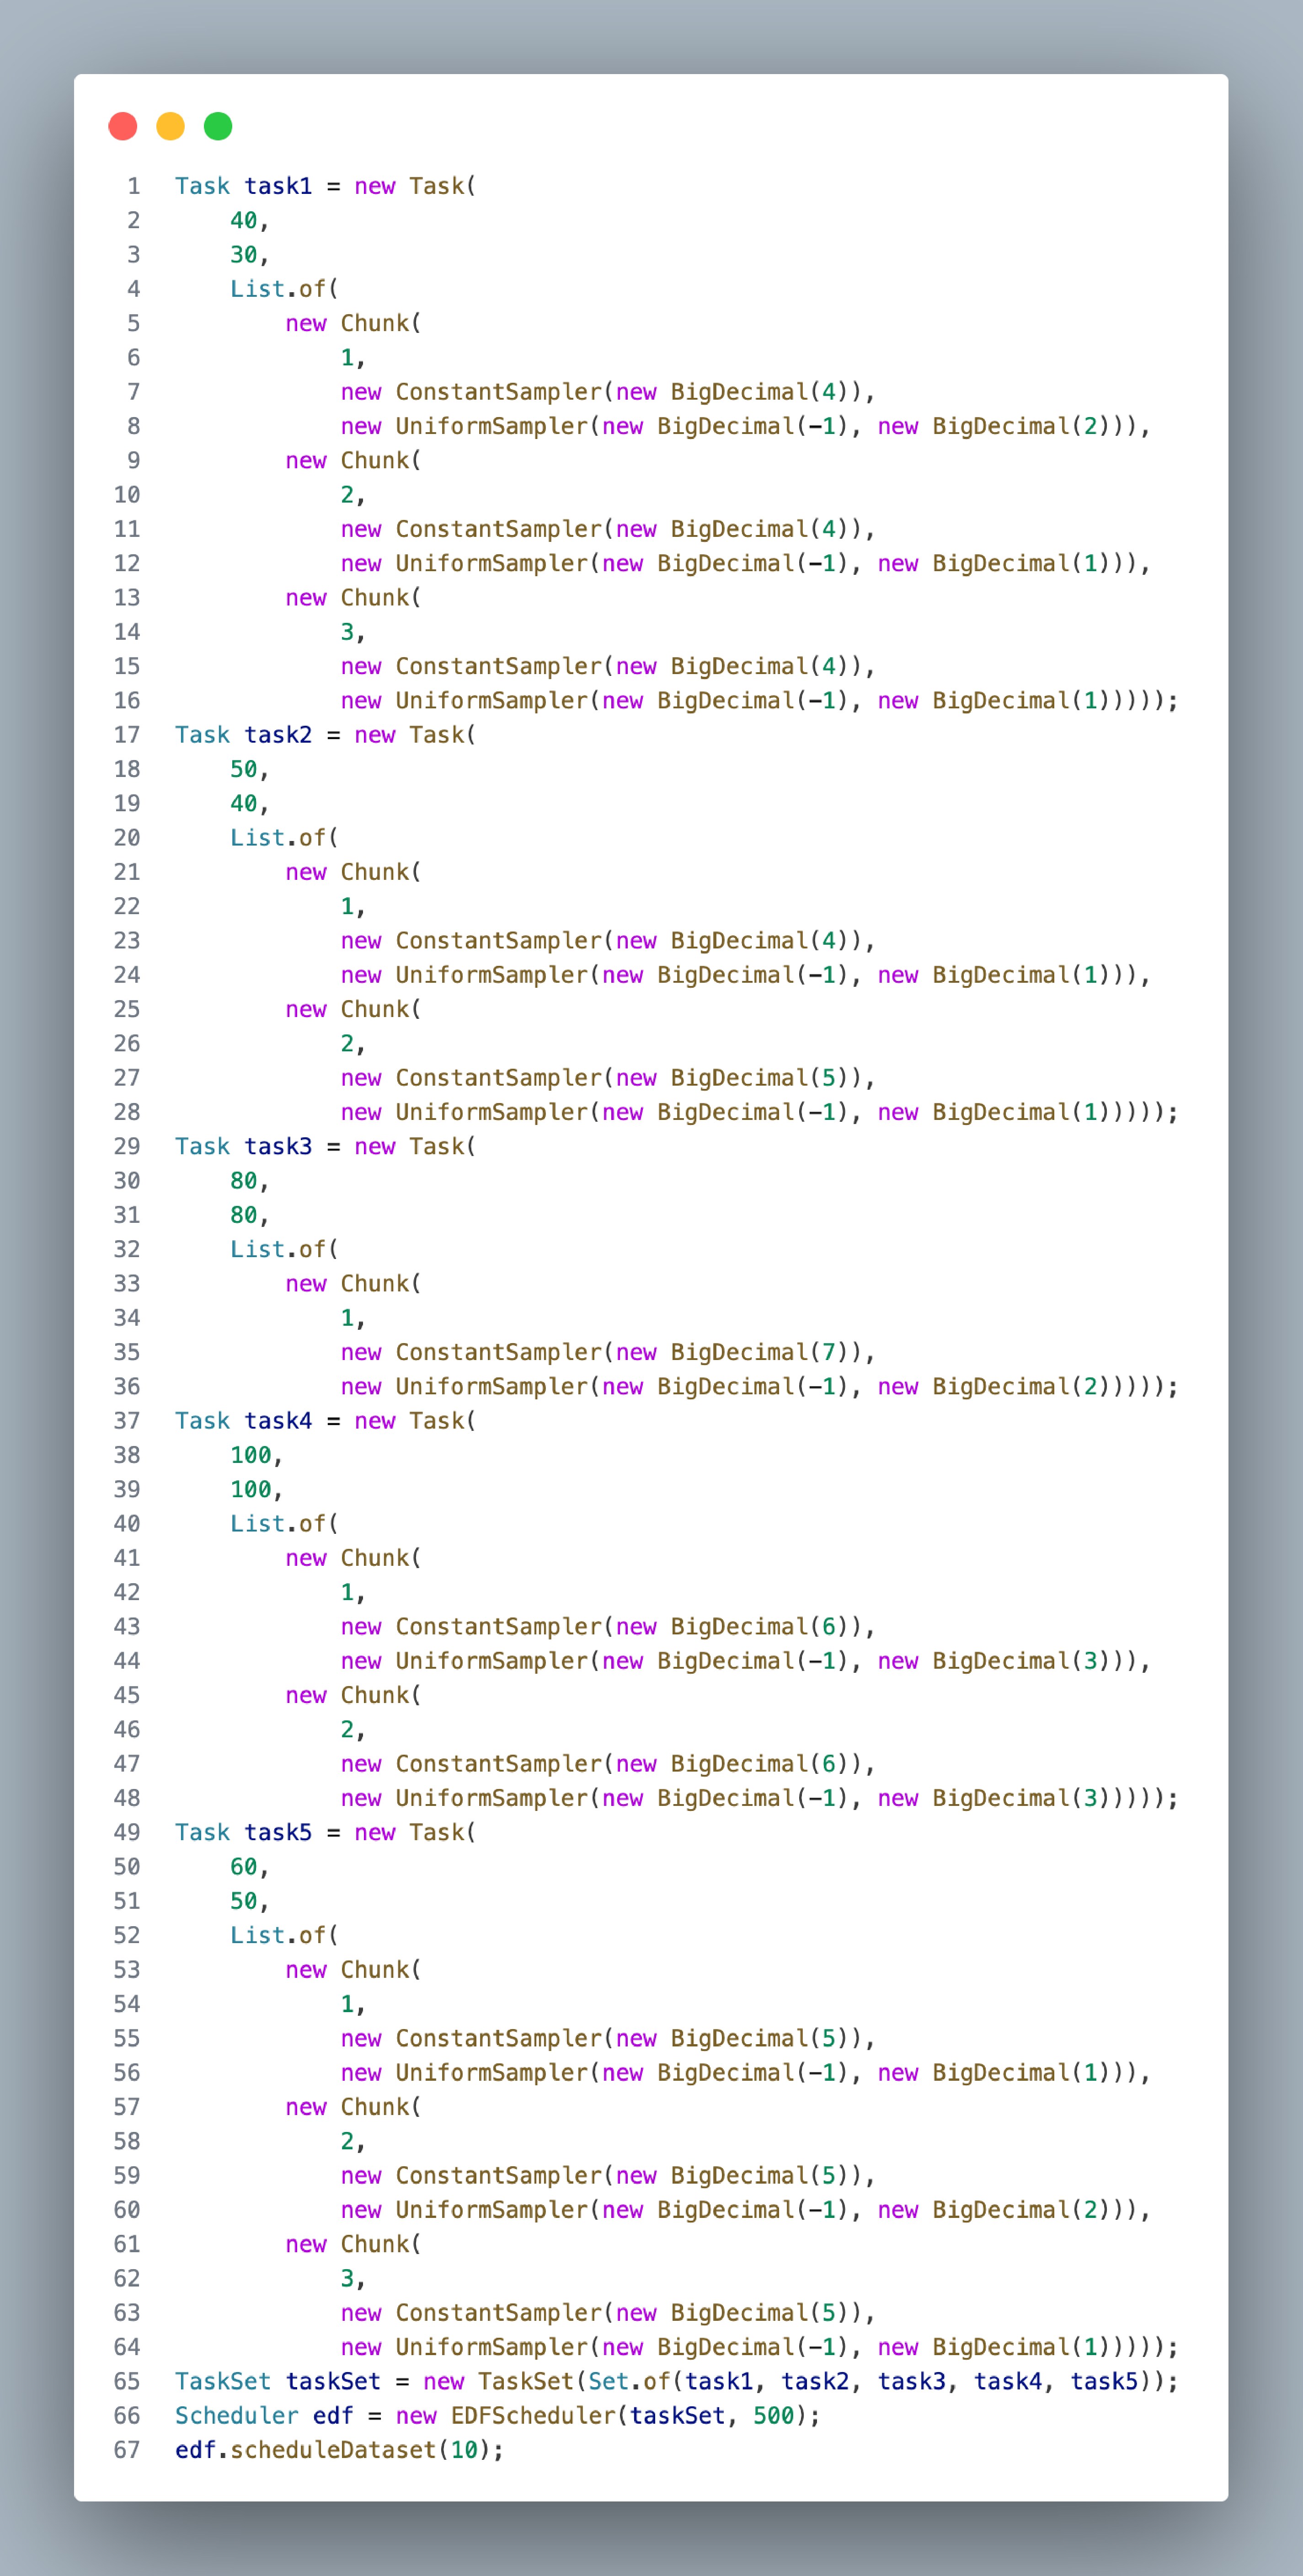
\includegraphics[width=.4\textwidth]{immagini/datasetEDF.pdf}
\centering
\caption{Taskset schedulato con EDF}
\label{fig:dataset1}
\end{figure}

Considerando la lunghezza delle tracce generate dalla simulazione, non si è potuto inserire il file \texttt{trace.log} in questo documento. Nel repository su \href{https://github.com/edoardosarri24/real-time-scheduling-simulator.git}{GitHub} è presente una cartella \texttt{output}, nella quale si può comunque osservare il risultato nel file \texttt{traceEDF.log}.

%%%%%%%%%%%%%%%%%%%%%%%%%%%%%%%%%%%%%%%%%%%%%%%%%%%%%%%%%%%%
\section{Taskset 2}
Il secondo taskset complesso, mostrato in Figura~\ref{fig:datasetRM}, è pensato per avere cinque task con due risorse condivise e per essere schedulato da Rate Monotonic sotto Priority Ceiling Protocol. Oltre alla stocasticità del tempo di esecuzione di ogni chunk, è stato inserito il fault a livello di Chunk per cui un chunk può non acquisire le risorse da usare con una probabilità del 20%.

\begin{figure}[htbp]
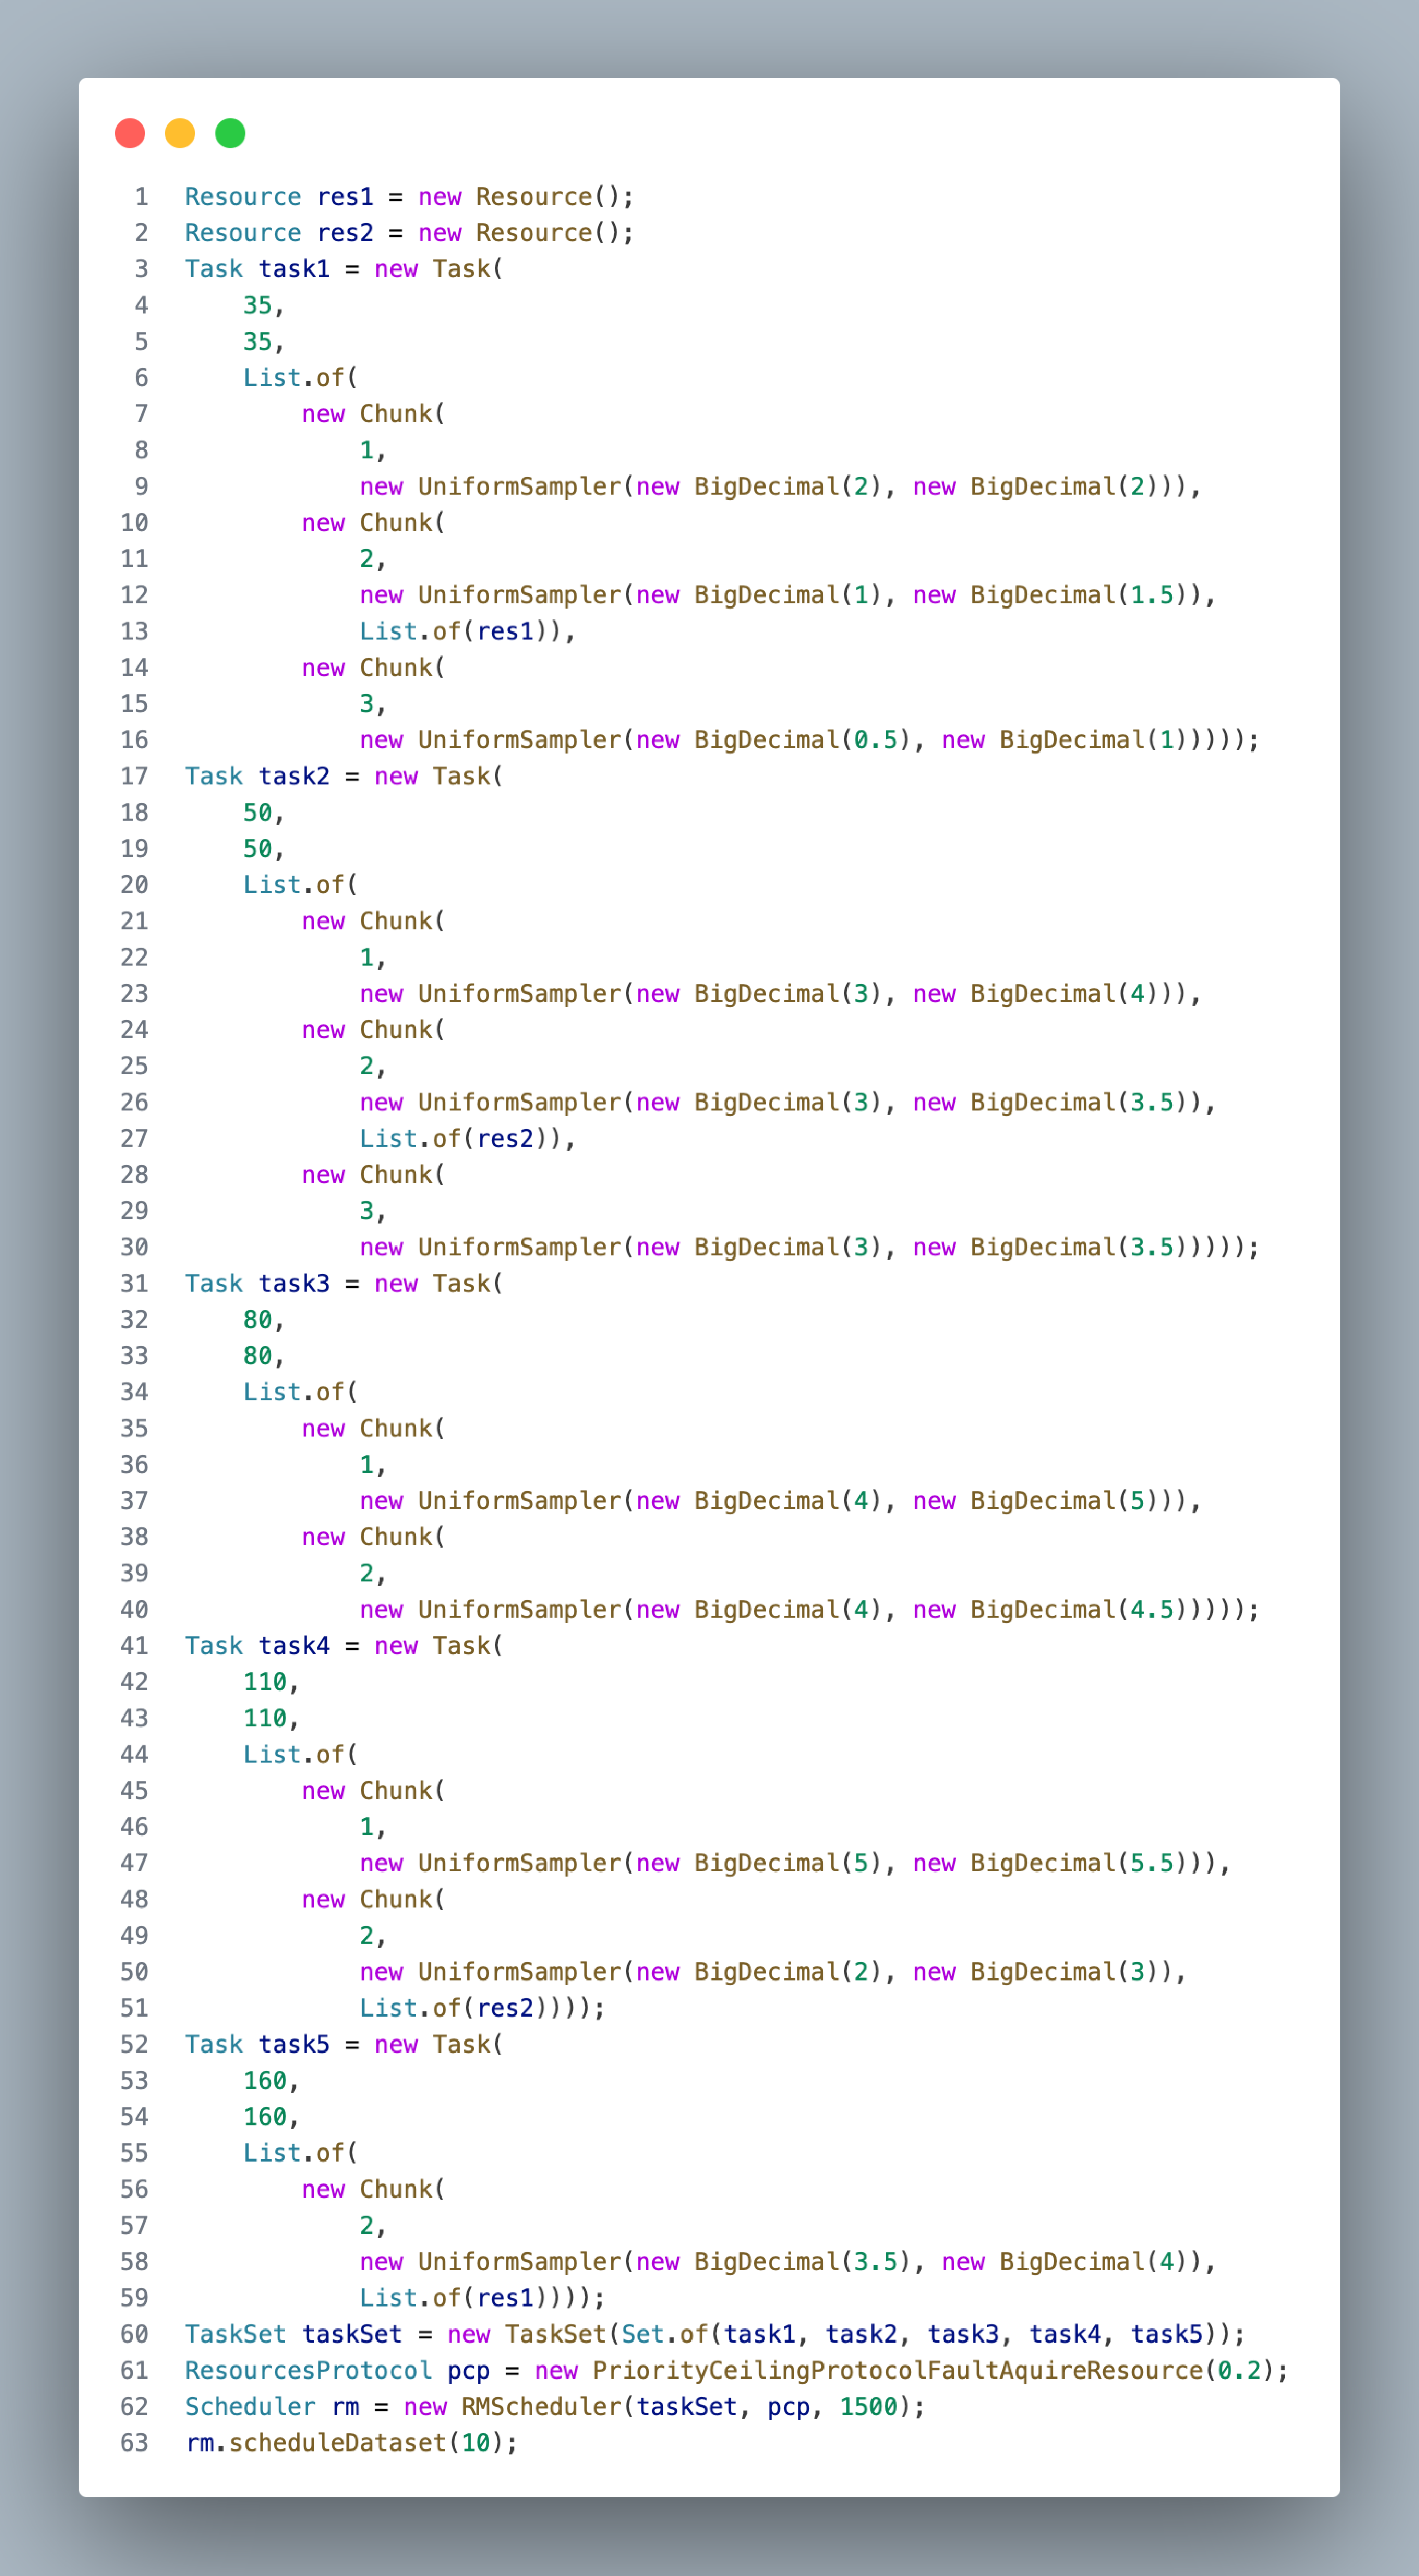
\includegraphics[width=.5\textwidth]{immagini/datasetRM.pdf}
\centering
\caption{Taskset schedulato con RM con risorse condivise sotto PCP}
\label{fig:datasetRM}

\end{figure}
Come per il caso precedente il file di log relativo a questa simulazione è nella cartella output sul repository di \href{https://github.com/edoardosarri24/real-time-scheduling-simulator.git}{GitHub} chiamato \texttt{traceRM.log}.